\documentclass[main.tex]{subfiles}
\begin{document}
    \section{Frame}
    The ladder frame is what we decided to go with, similar to our Competition 2 design. It consists of two L-Beams facing towards each-other with four I-Beam cross beams connecting them. There are a few major design changes that were made to adapt to changes in the pod subsystems. A longer frame was vital in the new design to accommodate the new friction drive propulsion system and the longer Eddy-Current Brakes. To avoid excessive torsional forces, and to simplify mounting of the friction drive and the shell, the frame was made narrower. For battery mounting, an additional flat plate crossmember was added parallel to the I-Beams. This flat plate was also vital for reducing deformities from the transverse forces of the EC Brakes.\\

    There was an investigation into using a honeycomb plate with sections cut out as the frame. While it would have been a very light alternative to the current ladder design, there were two major things holding us back from the decision. The first problem we ran into was the cost. The whole plate to be ordered would have been around \$4000, twice the anticipated expense for the frame. The other problem would be the complicated FEA associated with a honeycomb plate structure.  As a non isotropic material, the FEA would have taken a while to figure out and run. It was in our best interest to use our time to optimize the design of our ladder frame.\\

    The material used will be 7075 T6 for the I-beam crossmembers and 6061 T6 for the L-Beams. There was thought put into making the whole pod out of 6061 T6, similar to the competition 2 design, but due to the extreme forces from the EC-Brakes, the material had to be changed to 7075 T6 on the I-Beams. The 6061 T6 on the L-beams will be reasonable for our design, without increasing the cost of the frame too much.

    \subsection{Overall Design}
    \begin{figure}[H]
        \centering
        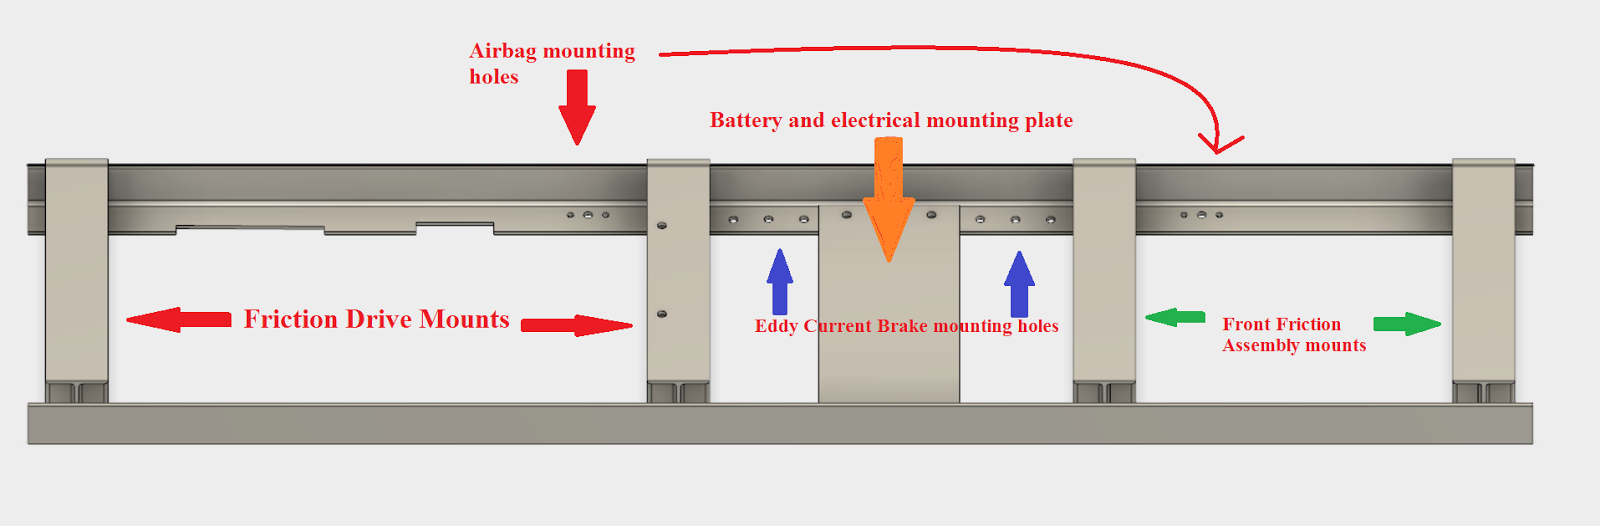
\includegraphics[width=\linewidth]{images/fig24}
        \caption{Caption needed}
    \end{figure}
    \begin{itemize}
        \item The mass of the whole frame will be approximately 25kg
        \item Dimensions would be 2.1m x 0.44m
    \end{itemize}
    Full cost breakdown, comments on manufacturability and production costs\\
    “A full Bill of Materials can be found in Appendix C.”

    \subsection{Structural}
    Modes of vibration (accounting for other subsystem masses)\\
    Dampening for those modes of vibration\\
    Speeds at which these modes of vibration can become a problem\\
    What are several reasonable and edge-case loading scenarios, and how does the FEA look for all of those? Justify your “reasonable” scenarios. If possible to simulate, how many cycles might it withstand?
    \begin{figure}[H]
        \centering
        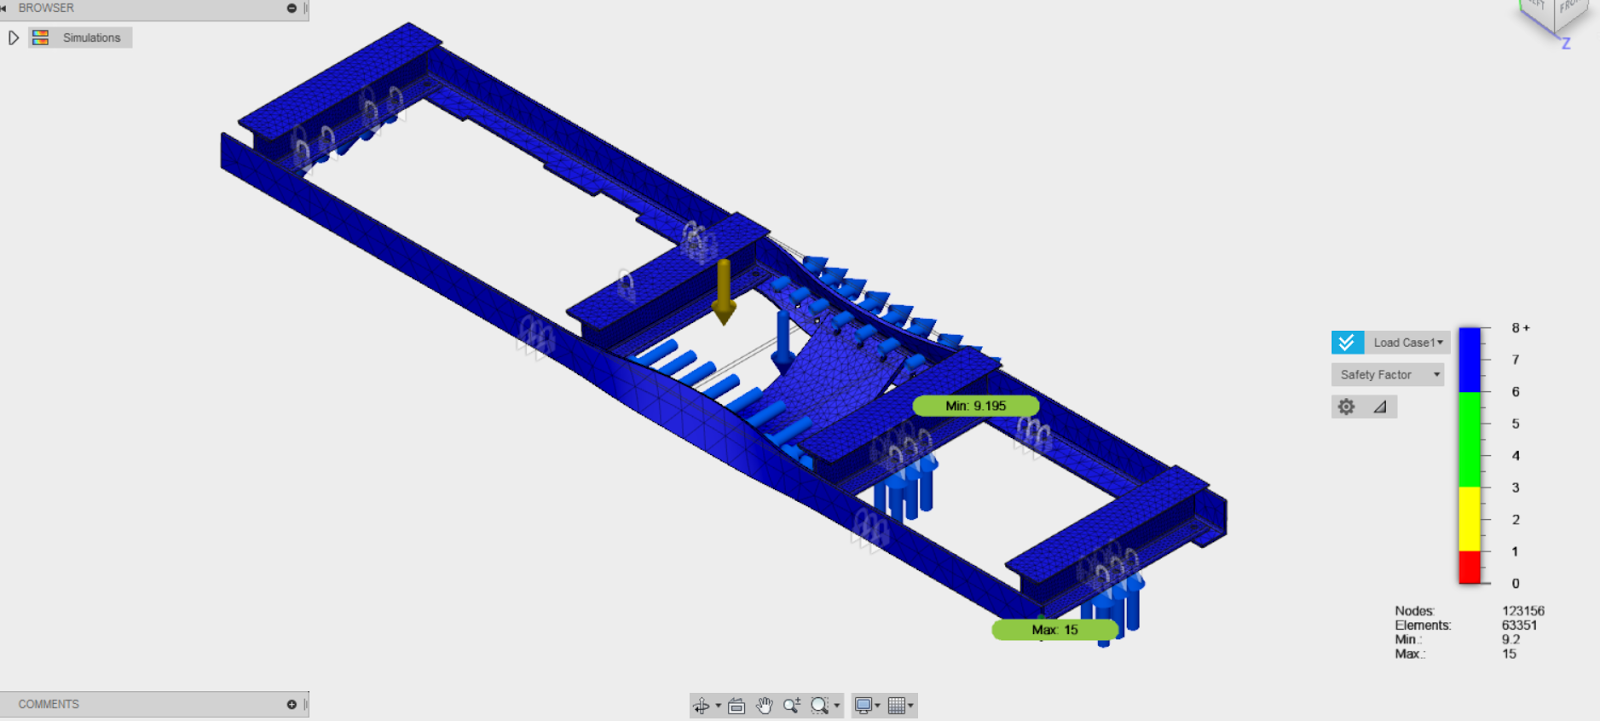
\includegraphics[width=\linewidth]{images/fig25}
        \caption{Caption needed}
    \end{figure}
    \begin{itemize}
        \item Profile if Braking was active, and friction drive was running
        \item Pod structural design cases: at a minimum, this shall include initial acceleration, nominal deceleration, and a reasonably foreseeable off-nominal crash (FEA)
    \end{itemize}

\end{document}
